\documentclass[a4paper,11pt]{ltjsarticle}
\usepackage{graphicx}
\usepackage{luatexja-fontspec}
\usepackage{caption}
\usepackage{amsmath,amssymb,bm,braket}
\usepackage[english]{babel}
\usepackage{multicol}
\usepackage{titlesec}
%\usepackage{gnuplot-lua-tikz}
\usepackage[top=20truemm,bottom=20truemm,left=20truemm,right=20truemm]{geometry}
\usepackage{array}
\usepackage{upgreek}
\usepackage{fancyhdr}
\renewcommand{\refname}{}
\usepackage{listings,jvlisting}
\usepackage{tikz}
\usepackage[thmmarks,amsmath]{ntheorem}
\usepackage[version=3]{mhchem}
\usetikzlibrary{external}
\tikzexternalize
\lstset{
  basicstyle={\ttfamily},
  identifierstyle={\small},
  commentstyle={\smallitshape},
  keywordstyle={\small\bfseries},
  ndkeywordstyle={\small},
  stringstyle={\small\ttfamily},
  frame={tb},
  breaklines=true,
  columns=[l]{fullflexible},
  numbers=left,
  xrightmargin=0pt,
  xleftmargin=3pt,
  numberstyle={\scriptsize},
  stepnumber=1,
  numbersep=1pt,
  lineskip=-0.5ex
}
\captionsetup[figure]{format=plain, labelformat=simple, labelsep=quad,labelfont=bf,name={Fig.}}
\captionsetup[table]{format=plain, labelformat=simple, labelsep=quad,labelfont=bf}
\parindent = 0pt
%[BoldFont=HGSMinchoE]{MSMincho}[BoldFont=HiraMinProN-W6]{HiraMinPro-W3}
\titleformat{\section}{\normalfont\fontsize{9}{10}\bfseries\fontspec{Times New Roman}}{\thesection.}{1em}{}
\usepackage[backend=biber,sorting=none,style=numeric,maxnames=99,minnames=1]{biblatex}
\addbibresource{utility/REFERENCES.bib}
\defbibheading{bibliography}[\refname]{%
  \section*{REFERENCES}%
  \vspace{-7pt}  % ここで空白を調整。お好みの値に変更してください。
}
\newfontfamily\subsectionfont{Times New Roman} % サブセクション用フォント
\titleformat{\subsection}
  {\normalfont\large\bfseries} % サブセクションのフォントを指定
  {\thesubsection}{1em}{}
\renewbibmacro{in:}{}
\renewbibmacro*{journal+issuetitle}{%
  \addcomma\space% カンマとスペースを追加
  \usebibmacro{journal}%
  \setunit*{\addspace}%
  \usebibmacro{volume+number+eid}%
  \setunit{\addspace}%
  \printfield{note}%
  \newunit
}
\renewbibmacro*{volume+number+eid}{
  \printfield{volume}%
  \setunit*{\addnbspace}%
  \printfield{number}%
  \setunit{\addcomma\space}%
  \printfield{eid}
}
\DeclareFieldFormat[article]{volume}{\textbf{#1}}
\DeclareFieldFormat[article]{pages}{#1}
\DeclareFieldFormat{journaltitle}{#1}
\usepackage{hyperref}
\renewenvironment{abstract}{\par\noindent}{\par}
%\pagenumbering{gobble}
\usepackage{docmute}
\usepackage{setspace}
\usepackage{titlesec} % 見出しのカスタマイズ用

% セクションのフォーマットをカスタマイズ
\titleformat{\section}
  {} % フォントサイズとスタイル
  {\Large\bfseries\thesection\ \ }               % 番号の前の内容(空白)
  {0em}            % 番号とタイトルの間の間隔
  {\Large\bfseries}


\theoremstyle{plain}
\theoremheaderfont{\normalfont\bfseries}
\theorembodyfont{\itshape}   % 本文を斜体に
\theoremseparator{.}         % タイトルと本文の区切りを「.」に設定
\newtheorem{definition}{Definition}
\begin{document}
\section{Surface Code}\label{surface_code}{
    \ \ \ The Surface Code, first introduced by Kitaev \cite{kitaev1997}, is the most promising error correction code for quantum computing. Using this code, universal computation can be performed with magic state distillation. In this section, we will first introduce the stabilizers of the Surface Code on the torus and then on the planar surface.

    \subsection{Surface Code on the Torus}{

        \begin{figure}[h]
            \centering
            \includegraphics[scale=0.20]{figure/torus.eps}
            \vspace{0pt}\caption{Physical qubits are located on the edges, while X-stabilizers and Z-stabilizers are placed on the vertices of the lattice.}
            \label{torus}
        \end{figure}

        \ \ \ Usually, the Surface Code is defined on a 1-genus torus, but it can also be defined on an $n$-genus torus in the same way. The lattice on the torus, shown in Fig.~\ref{torus}, has the following property:

        \begin{align}\label{euler_genus}
            V-E+F=2-2g
        \end{align}
        
        where $V$ is the number of vertices, $E$ is the number of edges, $F$ is the number of faces of the lattice on the torus, and $g$ is the genus. For $g = 1$, the 1-genus case, Eq.~\ref{euler_genus} equals $0$. We now introduce data qubits on the edges, $X$ stabilizers on the vertices, and $Z$ stabilizers on the faces, as shown in Fig.~\ref{local}. Incidentally, in Fig.~\ref{local}, the left and right sides are identical, and similarly, the upper and bottom sides are identical. Ancilla qubits for syndrome measurements are allocated at the center of the faces for the Zstabilizers and on the vertices for the X stabilizers.

        \begin{figure}[h]
            \centering
            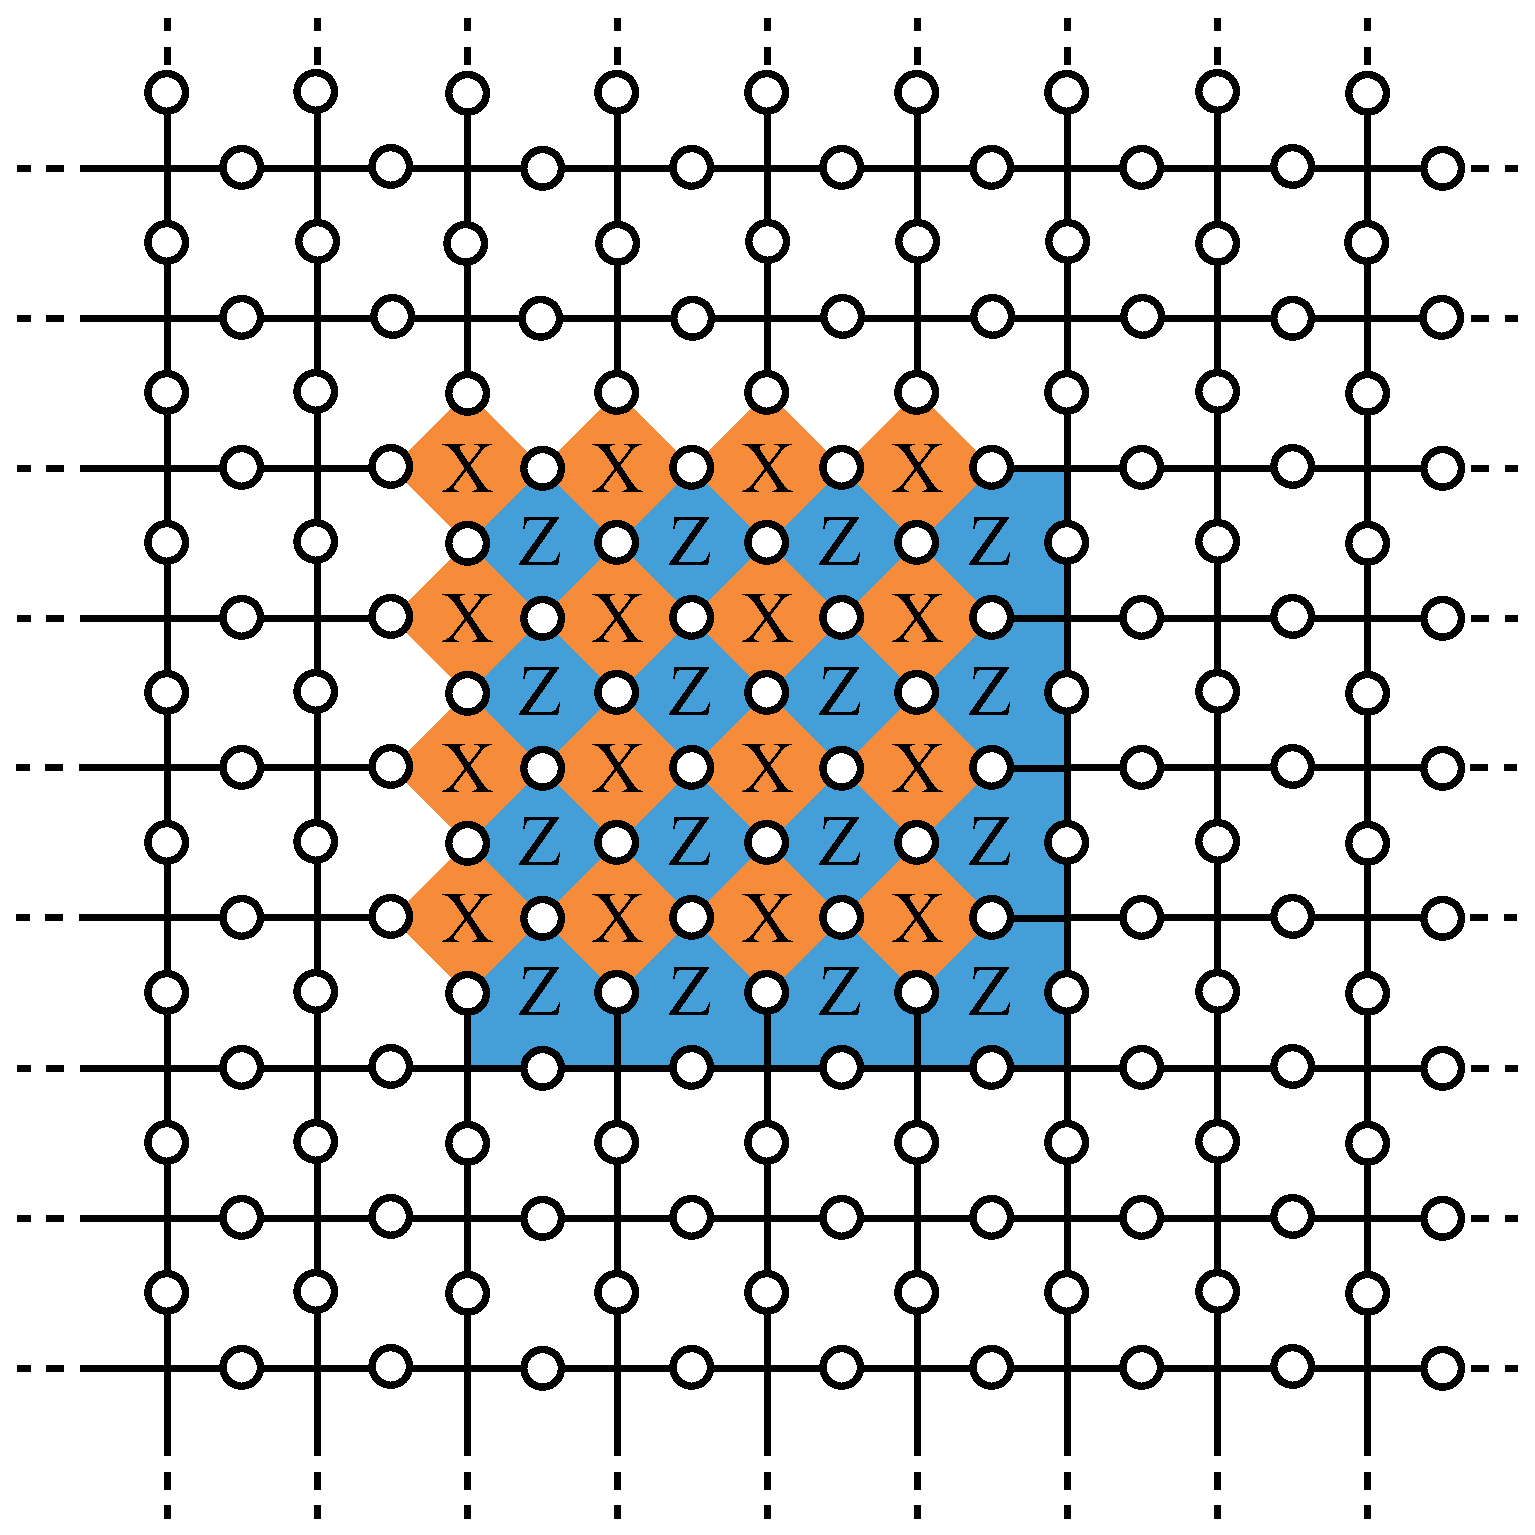
\includegraphics[scale=0.40]{figure/local.eps}
            \vspace{0pt}\caption{Physical qubits, X-stabilizer generators and Z-stabilizer generators on the torus. The right and left sides of the lattice are identical, and the top and bottom sides of the lattice are identical.}
            \label{local}
        \end{figure}
    
        In Fig.~\ref{local}, we show some of the stabilizers of the Surface Code, but others exist in the remaining parts of the lattice. Thus, we have $V - 1$ X stabilizer generators because the product of all X stabilizers on the vertices is the identity. From the same discussion, we have $F - 1$ Z stabilizer generators. Therefore, the number of logical qubits $k$ that can be encoded in the Surface Code is:

    \begin{align}
        k = E - (V - 1) - (F - 1) = 2
    \end{align} 

    using Eq.~\ref{euler_genus}. From these results, we can identify four logical operators corresponding to the non-trivial cycles on the torus. The logical operators are shown in Fig.~\ref{logical_operator}, where the subscripts 1 and 2 indicate the qubit numbers of the two logical qubits. From Fig.~\ref{logical_operator}, one can confirm that $L^i_XL^i_Z = -L^i_ZL^i_X$, that all logical operators commute with the stabilizers, and that the code distance is $\sqrt{n}$, which is the least weight of a logical operator. 

    \begin{figure}[h]
        \centering
        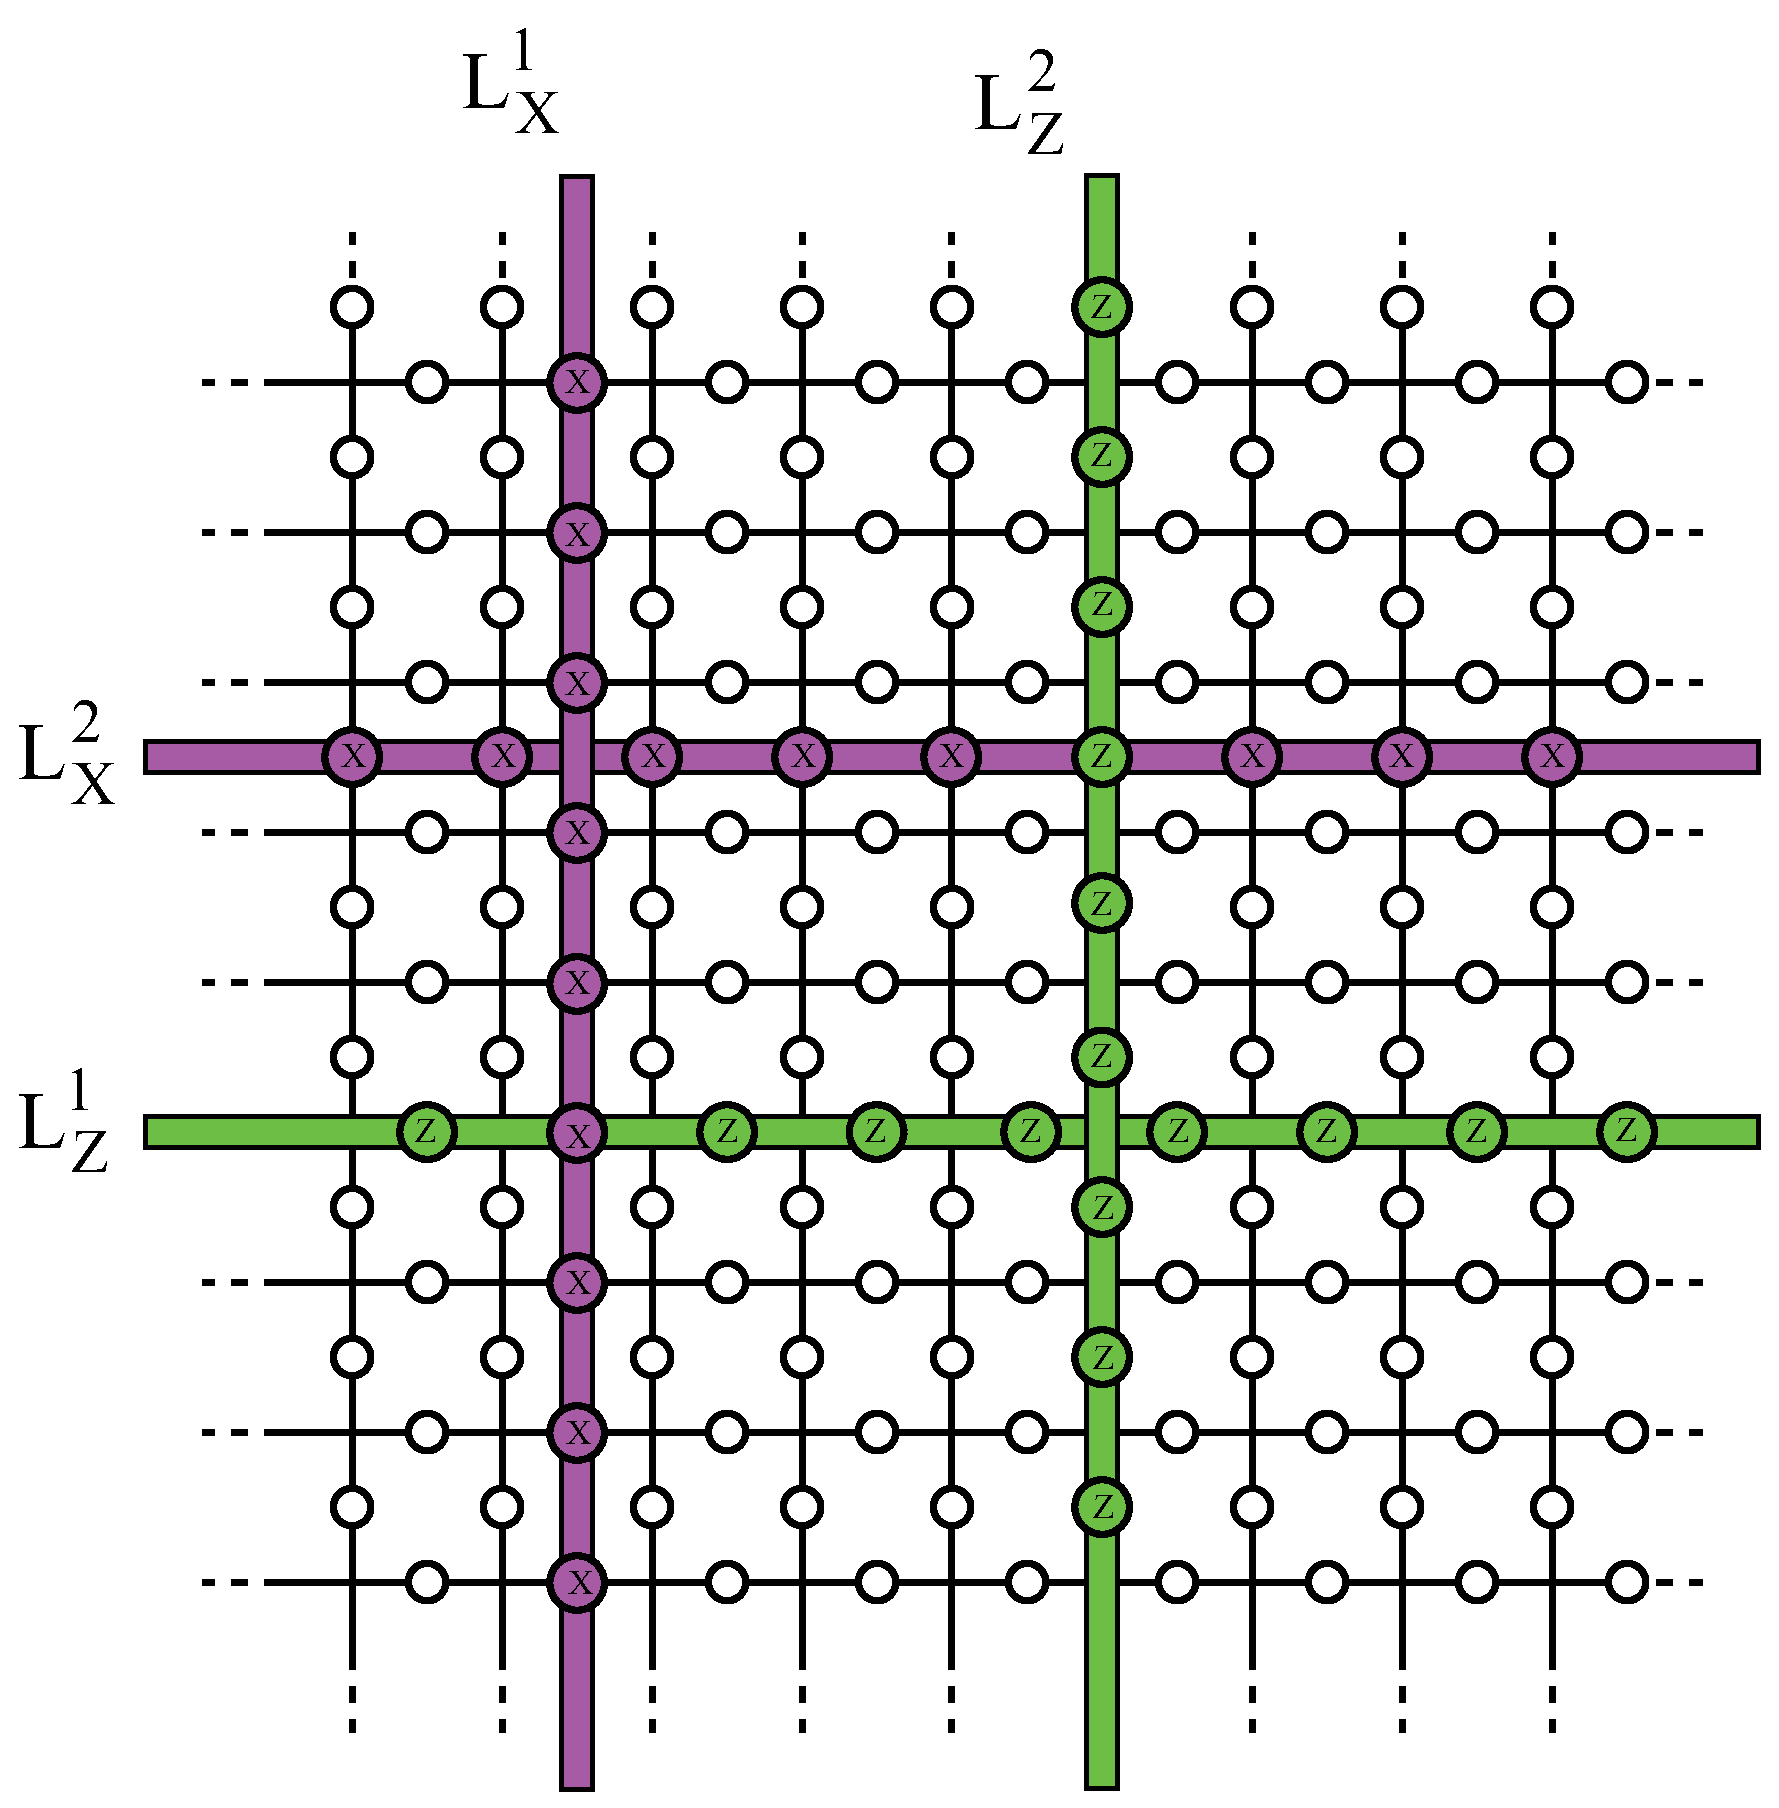
\includegraphics[scale=0.40]{figure/logical_operator.eps}
        \vspace{0pt}\caption{Logical operators of the surface code on the torus, which encode logical qubits. Purple lines represent logical X operators, and green lines represent logical Z operators.}
        \label{logical_operator}
    \end{figure}
    }


    \subsection{Surface Code on the Planar}{
        \ \ \ The Surface Code on the planar is different from that on the torus because it has boundaries, as shown in Fig.~\ref{planar}. One can observe that there exist 3-weight stabilizers at the boundaries. 

        \begin{figure}[h]
            \centering
            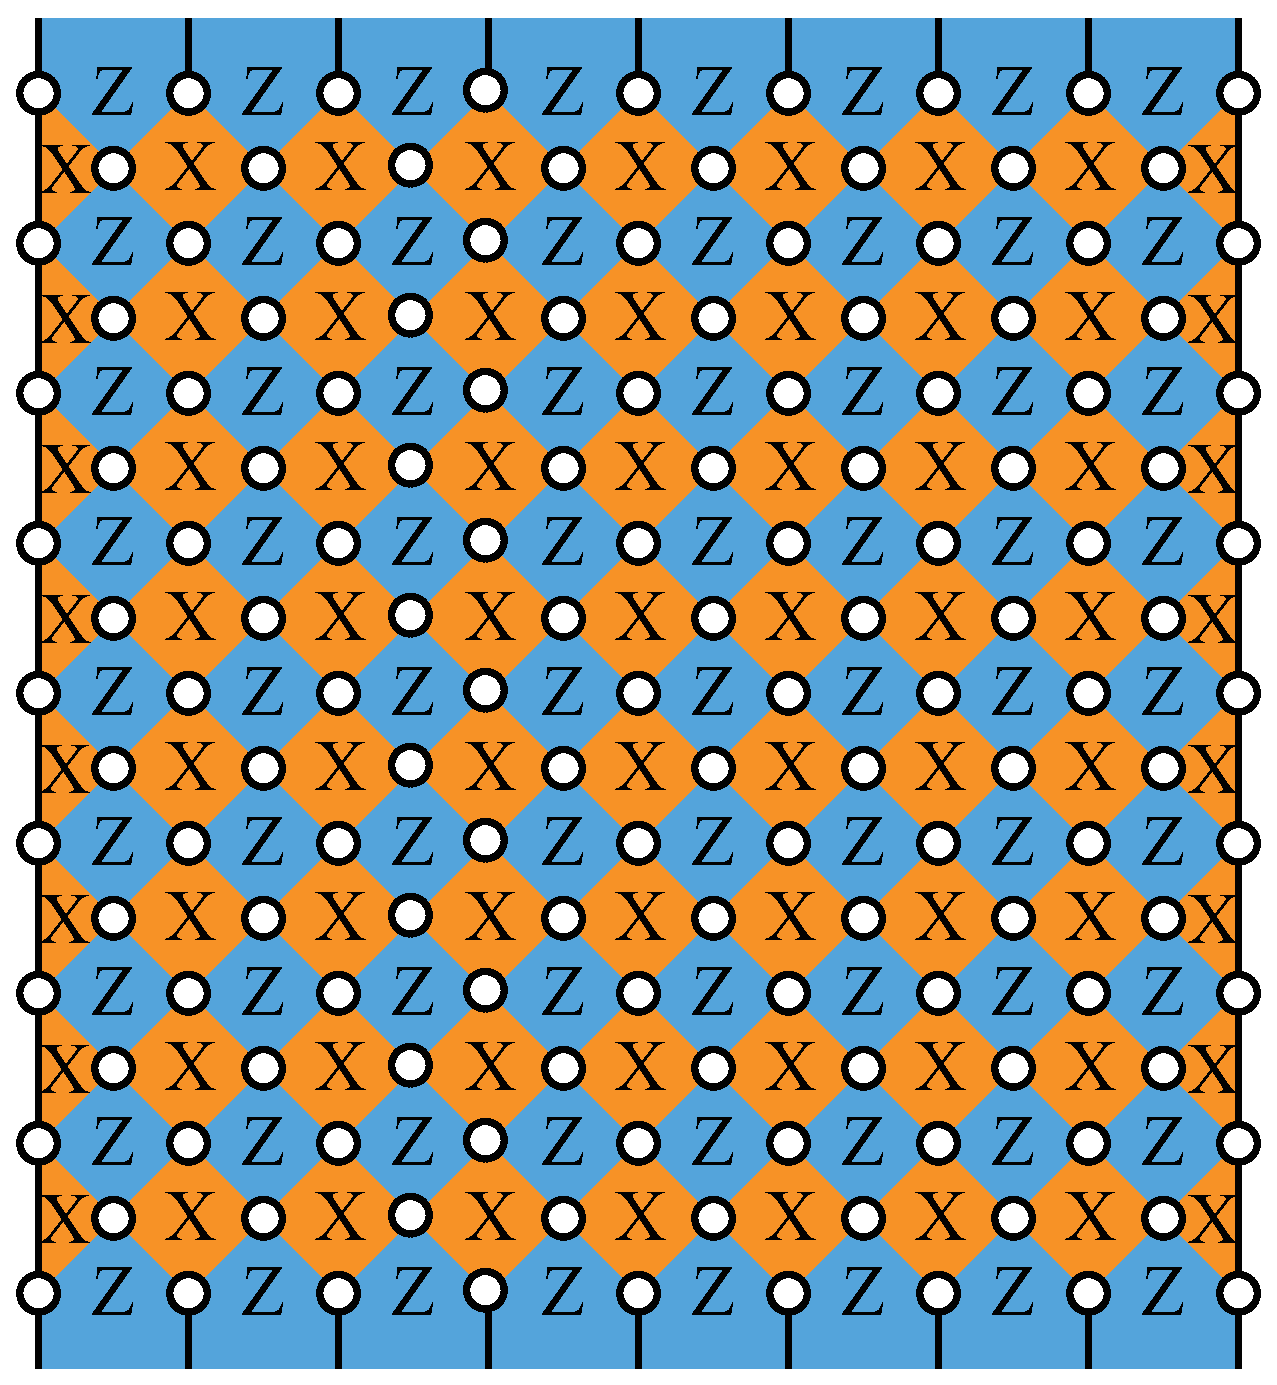
\includegraphics[scale=0.30]{figure/planar.eps}
            \vspace{0pt}\caption{Surface code on the plane. Orange shapes are X-stabilizers, and blue shapes are Z-stabilizers.}
            \label{planar}
        \end{figure}

        Additionally, the Surface Code on the planar can encode one logical qubit (Fig.~\ref{logical_operator_planar}). In the same way of the torus, one can confirm that code distance of the surface code in Fig.~\ref{logical_operator_planar} is $\sqrt{n}$ where there exists $n$ qubits. The two boundaries that are connected to each other by the logical Z operator are called rough boundaries, while the remaining boundaries are called smooth boundaries.

        \begin{figure}[h]
            \centering
            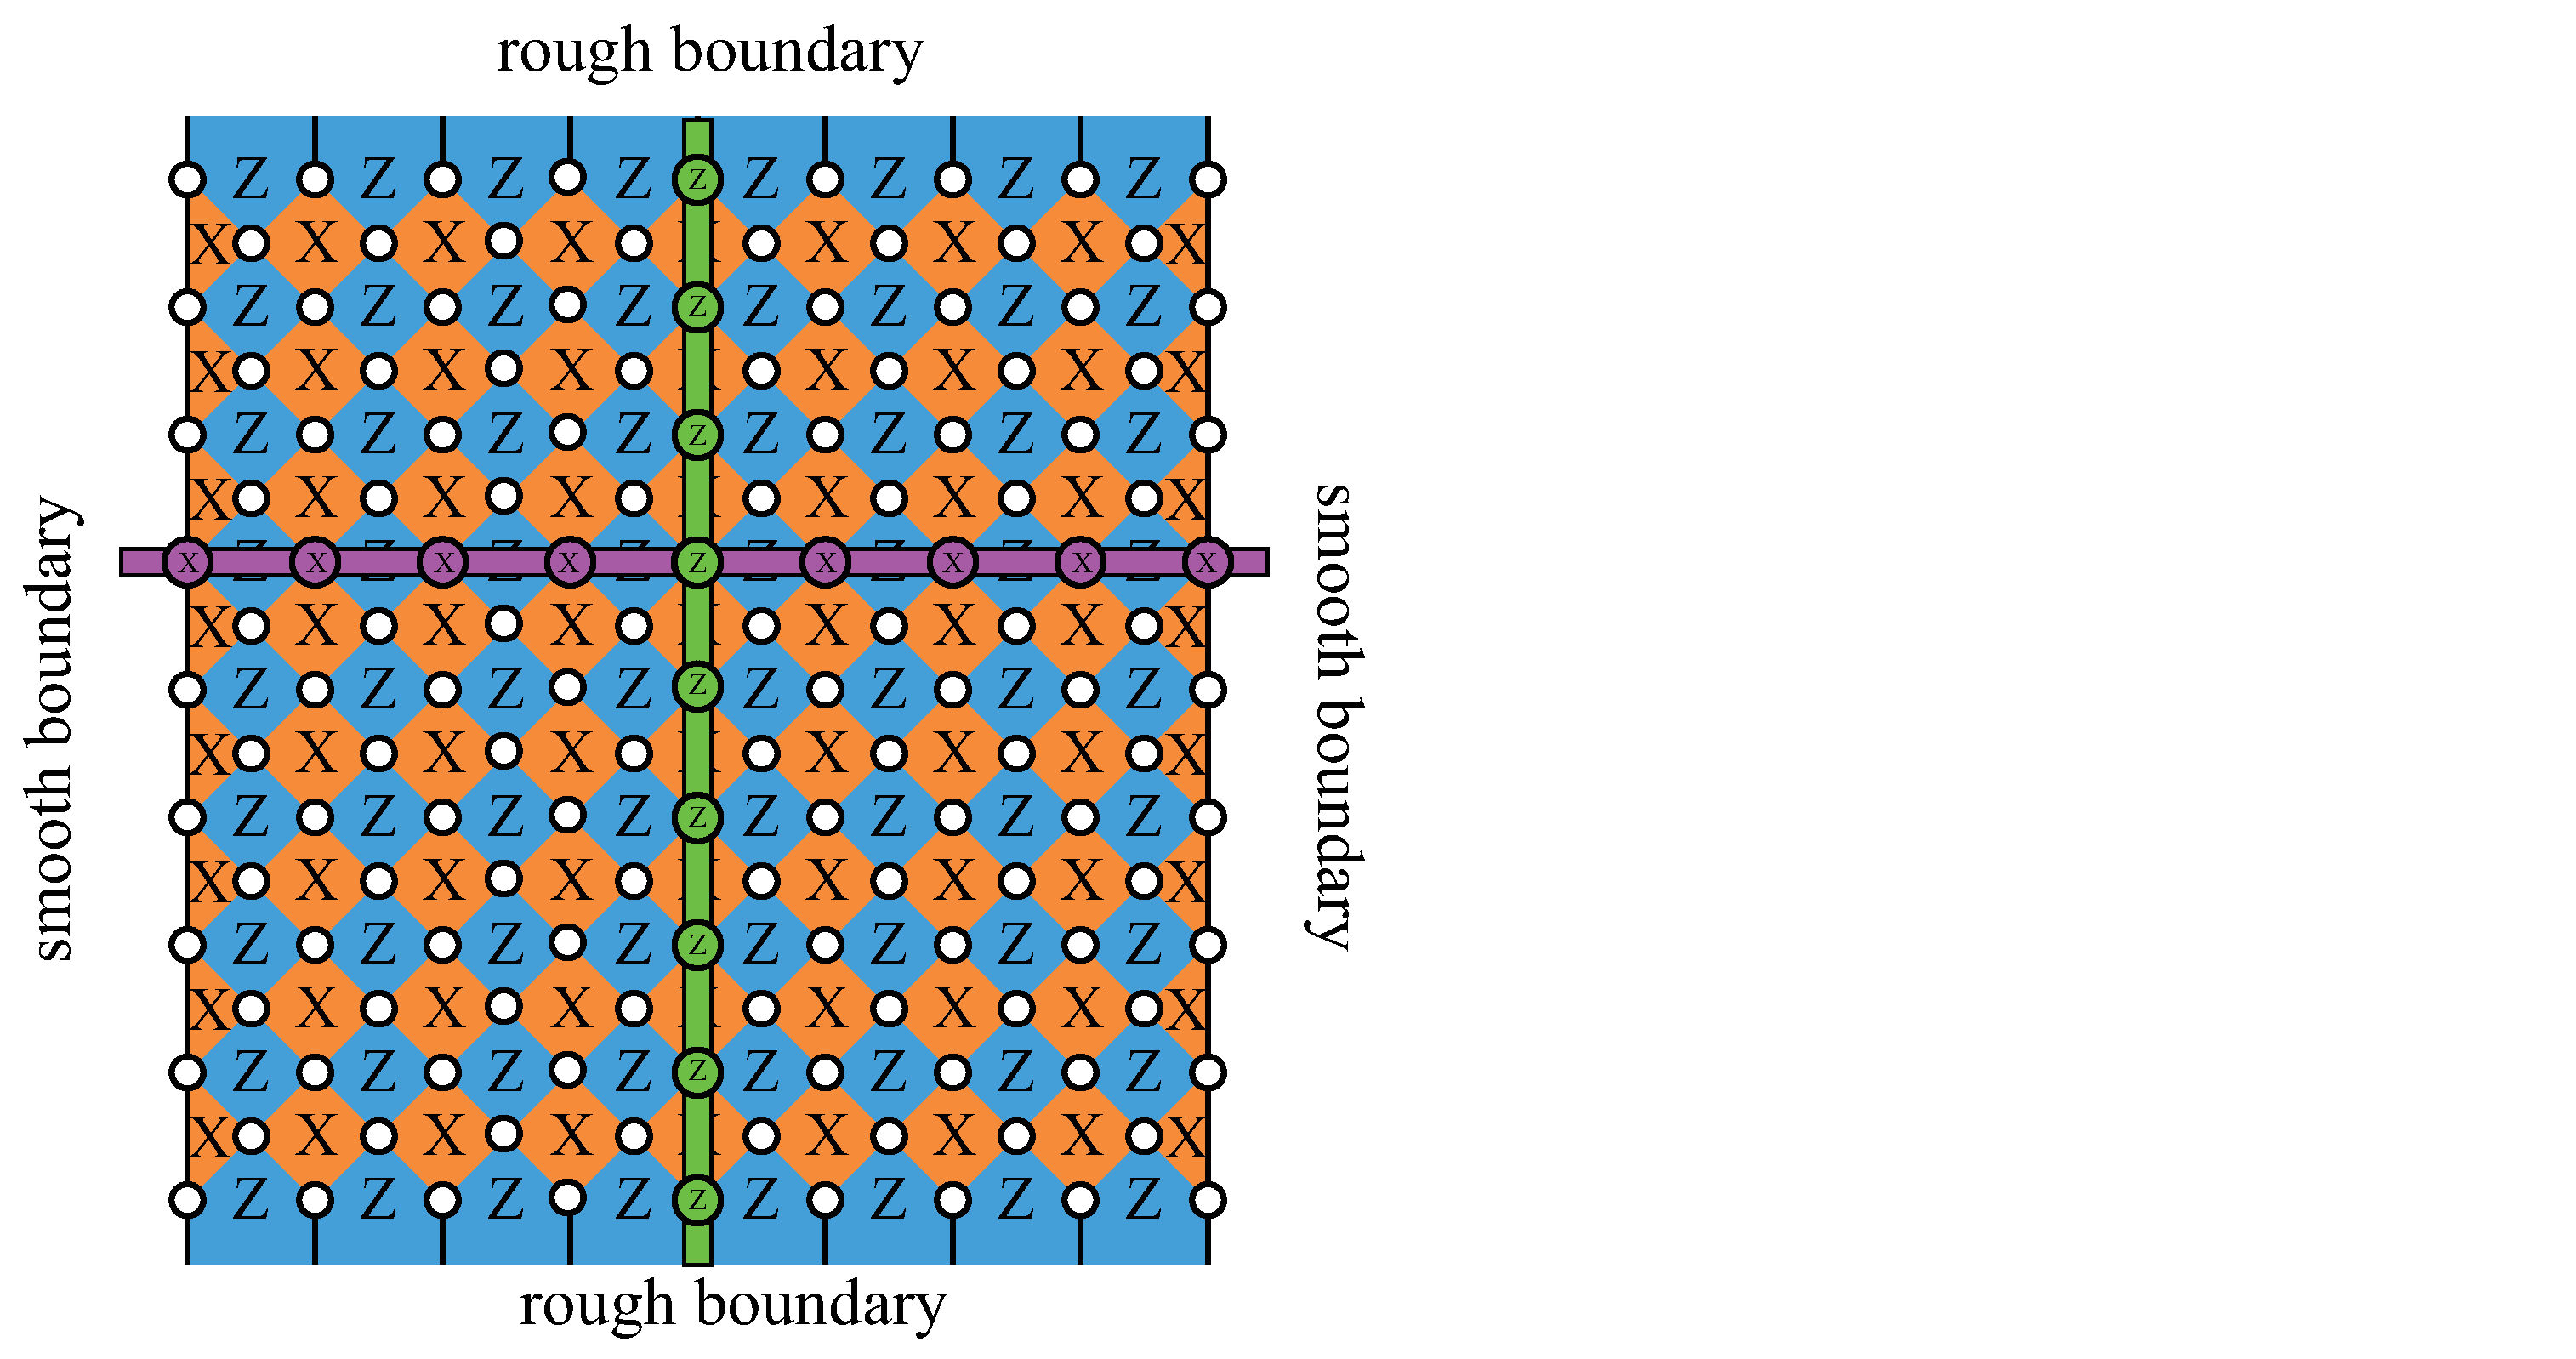
\includegraphics[scale=0.30]{figure/logical_operator_planar.eps}
            \vspace{0pt}\caption{A horizontal boundary, which consists of 3-weight Z-stabilizers, is called a rough boundary, and a vertical boundary, which consists of 3-weight X-stabilizers, is called a smooth boundary.}
            \label{logical_operator_planar}
        \end{figure}

        \ \ \ There exist excess qubits in the previous Surface Code. As shown in Fig.~\ref{rotated_surface_code}, we can cut along the green line, which contains both data qubits and ancilla qubits, trim off the excess parts, and rotate the lattice by 45 degrees to obtain the rotated Surface Code. With this modification, the code distance of the Surface Code is preserved by defining new logical operators on the rotated Surface Code that connect the rough boundaries or the smooth boundaries.


        \begin{figure}[h]
            \centering
            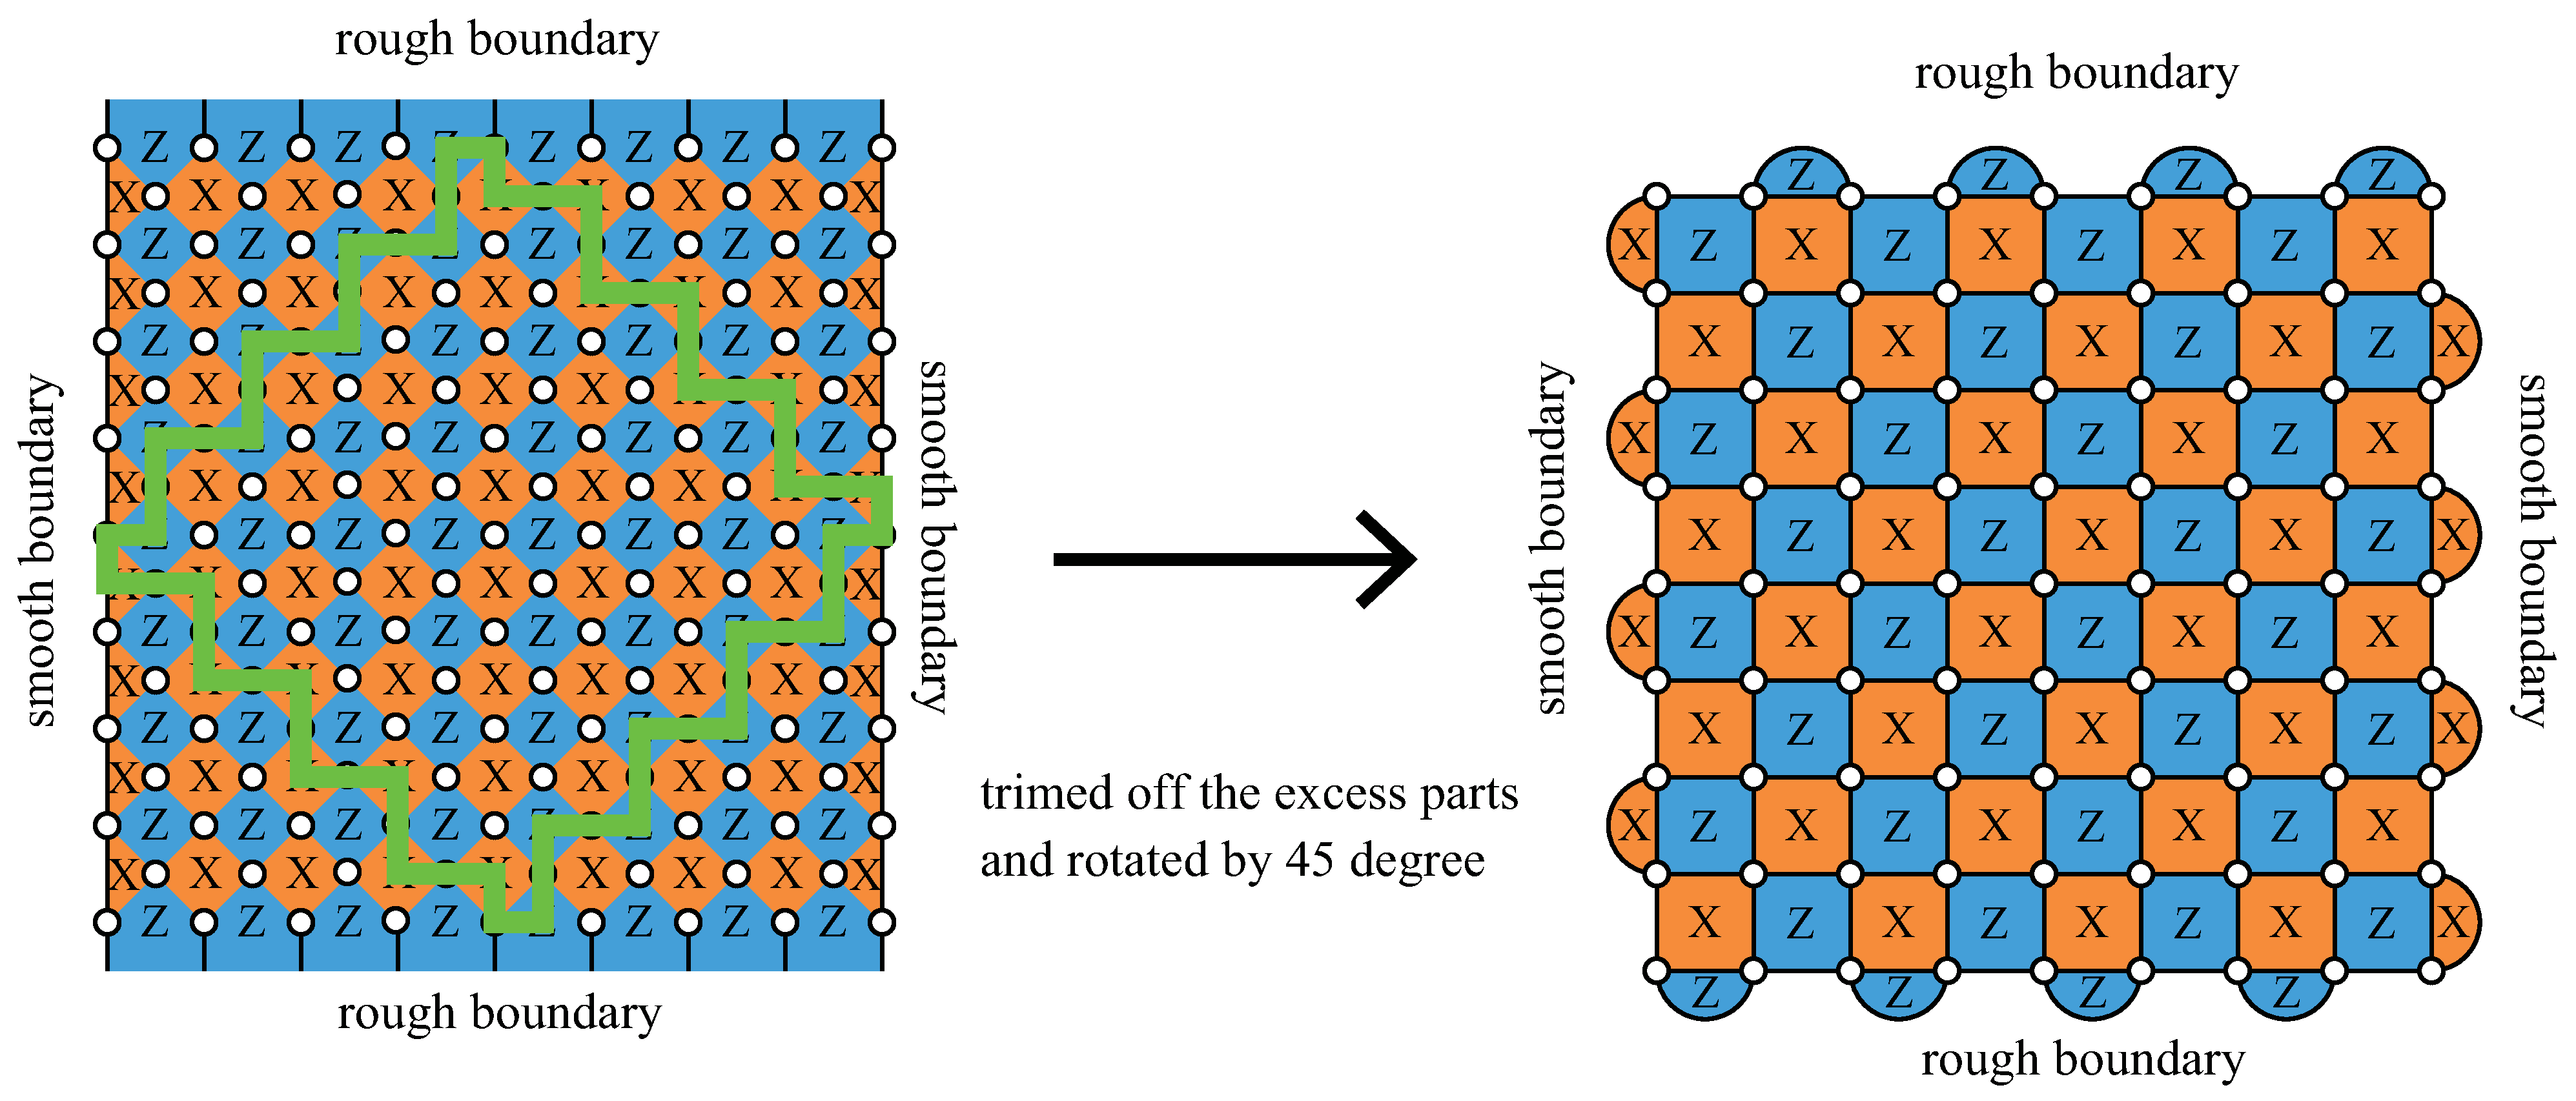
\includegraphics[scale=0.25]{figure/rotated_surface_code.eps}
            \caption{By trimming the excess parts of the previous surface code, we obtained a new surface code while preserving its distance.}
            \label{rotated_surface_code}
        \end{figure}

        
    }
}
\end{document}